%%% Add [final] option to the report class to switch between draft and final version of the report
%%% Use [narrowmargin] to enable narrow margins - this may impair readability.
\documentclass[a4paper, 10pt]{include/compassreport}   %Or compasslargereport if chapters are required.

\usepackage{times}
\usepackage{graphicx,caption}

\graphicspath{{figures/}}

\usepackage[cmex10]{amsmath}
\usepackage{amssymb}
%\usepackage{amsfonts}
%\fontencoding{T4}
%\usepackage{marvosym}
%\usepackage{wasysym}
\usepackage{ifthen}
\usepackage{tabularx}
\usepackage{longtable}
\usepackage{listings}
\usepackage{wrapfig}
\usepackage{cmllisting}
\usepackage{subcaption}

%remove red boxes on links
\hypersetup{%
    pdfborder = {0 0 0}
}

%%Figures
\usepackage{tikz,bm,color}
\usetikzlibrary{shapes,arrows}
\usetikzlibrary{positioning,fit,calc}
\usetikzlibrary{arrows}
\usetikzlibrary{decorations.pathreplacing,patterns}
%\usepackage{color}
%\usepackage{float}
%\restylefloat{table}
% correct bad hyphenation here
%\hyphenation{op-tical net-works semi-conduc-tor}

\def\sectionautorefname{Section}
\def\subsectionautorefname{Subsection}
\def\subsubsectionautorefname{Subsection}

\DeclareMathSymbol{\B}{\mathalpha}{AMSb}{"42}
\DeclareMathSymbol{\I}{\mathalpha}{AMSb}{"49}
\DeclareMathSymbol{\N}{\mathalpha}{AMSb}{"4E}
\DeclareMathSymbol{\Pwr}{\mathalpha}{AMSb}{"50}
\DeclareMathSymbol{\Q}{\mathalpha}{AMSb}{"51}
\DeclareMathSymbol{\R}{\mathalpha}{AMSb}{"52}
\DeclareMathSymbol{\Z}{\mathalpha}{AMSb}{"5A}
\DeclareMathSymbol{\Sol}{\mathalpha}{AMSb}{"53}

\newcommand{\obsv}[1]{{\cal O}(#1)}
\newcommand{\ctrl}[1]{{\cal C}(#1)}
\newcommand{\vdot}[1]{\stackrel{.}{#1}}
\newcommand{\power}{\mathbf{P}}

\newcommand{\HS}{{\mathcal H}}

\newcommand{\Interval}{\I}

\newcommand{\ist}{\mbox{{\tt true}}}
\newcommand{\isf}{\mbox{{\tt false}}}
\newcommand{\emptytrace}{\langle~\rangle}
\newcommand{\abegin}{\mathbf{begin}}
\newcommand{\aend}{\mathbf{end}}
\newcommand{\alet}{\mathbf{let}}
\newcommand{\aendlet}{\mathbf{endlet}}
\newcommand{\ain}{\mathbf{in}}
\newcommand{\afor}{\mathbf{for}}
\newcommand{\adownto}{\mathbf{downto}}
\newcommand{\aforall}{\mathbf{foreach}}
\newcommand{\awhile}{\mathbf{while}}
\newcommand{\ado}{\mathbf{do}}
\newcommand{\aenddo}{\mathbf{enddo}}
\newcommand{\acontinue}{\mathbf{continue}}
\newcommand{\aif}{\mathbf{if}}
\newcommand{\athen}{\mathbf{then}}
\newcommand{\aelse}{\mathbf{else}}
\newcommand{\aelseif}{\mathbf{elseif}}
\newcommand{\aendif}{\mathbf{endif}}
\newcommand{\ainout}{\mathbf{inout}}
\newcommand{\aout}{\mathbf{out}}
\newcommand{\aprocedure}{\mathbf{procedure}}
\newcommand{\afunction}{\mathbf{function}}
\newcommand{\abreak}{\mathbf{break}}
\newcommand{\Sup}[1]{\overline{#1}}
\newcommand{\Inf}[1]{\underline{#1}}


\newcommand{\taba}{\hspace*{3mm}}
\newcommand{\tabb}{\hspace*{6mm}}
\newcommand{\tabc}{\hspace*{9mm}}
\newcommand{\tabd}{\hspace*{12mm}}
\newcommand{\tabe}{\hspace*{15mm}}
\newcommand{\tabf}{\hspace*{18mm}}
\newcommand{\tabg}{\hspace*{21mm}}

\newcommand{\gca}[1]{{{#1}^{\vartriangleright}}}
\newcommand{\gcb}[1]{{{#1}^{\vartriangleleft}}}
\newcommand{\gclr}{{{\vartriangleleft\atop\longleftarrow}\atop
                   {\longrightarrow\atop\vartriangleright}}}

\newcommand{\dontshow}[1]{}


\newcommand{\Nat}{{\mathbb N}}
\newcommand{\Real}{{\mathbb R}}

\newcommand{\trans}{\longrightarrow}
\newcommand{\transp}{\longrightarrow_{\power}}
\newcommand{\transl}{\longrightarrow_{L}}
\newcommand{\transg}{\longrightarrow_{G}}
\newcommand{\transcfg}[1]{\stackrel{#1}{\longrightarrow}_{CFG}}
\newcommand{\isdefd}{=_{\mbox{\footnotesize def}}}
\newcommand{\equivdef}{\equiv_{\mbox{\footnotesize def}}}
\newcommand{\mitem}{\mbox{\em M-Item}}
\newcommand{\fun}{\rightarrow}
\newcommand{\pfun}{\not\rightarrow}
\newcommand{\currt}{\hat{t}}

\newcommand{\dom}{\mbox{dom}}
\newcommand{\ran}{\text{ran}}

\newcommand{\sigmaa}{\sigma_A}
\newcommand{\strictimplies}{\stackrel{\bullet}{\Rightarrow}}


\newtheorem{definition}{Definition}
\newtheorem{property}{Property}
\newtheorem{lemma}{Lemma}
\newtheorem{theorem}{Theorem}

\newcommand{\todo}[2]{\marginpar{\textbf{#1:} #2}}

\newboolean{showcomments}
%\setboolean{showcomments}{true}
\setboolean{showcomments}{false}

\newcommand{\com}[1]{\ifthenelse{\boolean{showcomments}}{
           \bigskip
           \noindent
           \framebox
       {\parbox{\textwidth}{
           {\sf #1}
           }}}{}}
           

\newcounter{examplectr}[section]
\newenvironment{example}[1] 
{
{\refstepcounter{examplectr}
\bf Example~\thesection.\theexamplectr.\label{#1}}
}
{

}

\lstdefinestyle{shstyle}{basicstyle=\footnotesize\ttfamily,
			frame=trbl, 
			showstringspaces=false,  
			captionpos=b,
			frameround=tttt, 
			aboveskip=5mm, 
			belowskip=5mm,
			breaklines=true,
			tabsize=4,
			framexleftmargin=0mm, 
			framexrightmargin=0mm}
\lstnewenvironment{shell}{\lstset{style=shstyle}\lstset{language=sh}}{}


\def\draftnote#1{\smallskip\noindent\hspace*{-3em}\framebox{\color{red}\begin{minipage}{\textwidth}#1\end{minipage}}\smallskip\par}

\def\filepath{\nolinkurl}


\reportnumber{DXX}
\reporttitle{CML Interpreter Design Document}
\shortreporttitle{Simulator/Animator}  %To use if report title is too long for header

%%% Set document release class as appropriate
%%% e.g. Public, Restricted, Programme Participant
\reportstatus{Public}


%%% If document is a deliverable, this flag should be commented out 
%%% e.g. %\technotetrue
%%% If report is a technical report, leave uncommented
%%% e.g. \technotetrue
\technotetrue % Comment out as appropriate

\submissiondate{Month Year}
\contributors{
  Anders Kaels Malmos, AU 
}
\editors{
  Peter Gorm Larsen, AU
}
\reviewers{}


%% Version details  
% #1: version
% #2: date
% #3: author
% #4: description
\addversion{0.1}{25-04-2013}{Anders Kaels Malmos}{Initial document version}
\addversion{0.2}{06-03-2014}{Anders Kaels Malmos}{Added introduction and domain description}
% \addversion{0.2}{dd-mm-yyyy}{Richard Payne}{Second version}

\begin{document}
\maketitle


%%%% Document abstract page %%%% 
\section*{Abstract}
\label{sec:abstract}

This document describes the overall design of the CML
simulator/animator and provides an overview of the code structure
targeting developers.

\newpage

%%%% Document table of contents page %%%% 
\tableofcontents
\newpage

%%%% Document Content %%%% 
%% \chapter{Chapter Title} %% if compasslargereport is in use
\section{Introduction}\label{sec:introduction}
This document is targeted at developers and describes the overall
design of the CML simulator, it is not a detailed description of each
component. This kind of documentation is done in Javadoc and can be
generated automatically from the code. It is assumed that common
design patterns are known like \ref{GOF}.

\subsection{Problem Domain}\label{sec:problem_domain}
The goal of the interpreter is to enable simulation/animation of a
given CML \ref{cml syntax} model and be able to visualize this in the
Eclipse IDE Debugger. CML has a UTP semantics defined in \ref{cml
semantics} which dictates how the interpretation progresses. Therefore, the
overall goal of the CML interpreter is to adhere to the semantic
rules defined in those documents and to somehow visualize this in the
Eclipse Debugger.

In order to get a high level understanding of how CML is interpreted
without knowing all the details of the semantics and the
implementation of it. A short illustration of how the interpreter
represents and progresses a CML model is given below. 

In listing \ref{lst:cmlexample} a CML model consisting of three CML
processes is given. It has a R (Reader) process which reads a value from
the inp channel and writes it on the out channel. The W (Writer)
process writes the value 1 to the inp channel and finishes. The
S (System) process is a parallel composition of these two processes where
they must synchronize all events on the inp channel.

\begin{cml}[caption=A process S composed of a parallel composition of a reader and writer process,tabsize=2, label={lst:cmlexample}]
channels
inp : int
out : int

process W = 
begin
 @ inp!1 -> Skip 
end

process R = 
begin
 @ inp?x -> out!x -> Skip 
end

process S = W [|{$inp$}|] R
\end{cml}

The interpretation of a CML model is done through a series of
steps/transitions starting from a given entry point. In figure
\ref{fig:cmlmodel_first_step} the first step in the interpretation of
the model is shown, it is assumed that the S process is given as the
starting point. Process are represented as a circle along with its
current position in the model. Each step of the execution is split up
in two phases, the inspection phase and the execution phase. The
dashed lines represents the environment (another actor that invokes
the operation e.g a human user or another process) initiating the phase.

 \begin{minipage}{1\linewidth} 
  \centering %
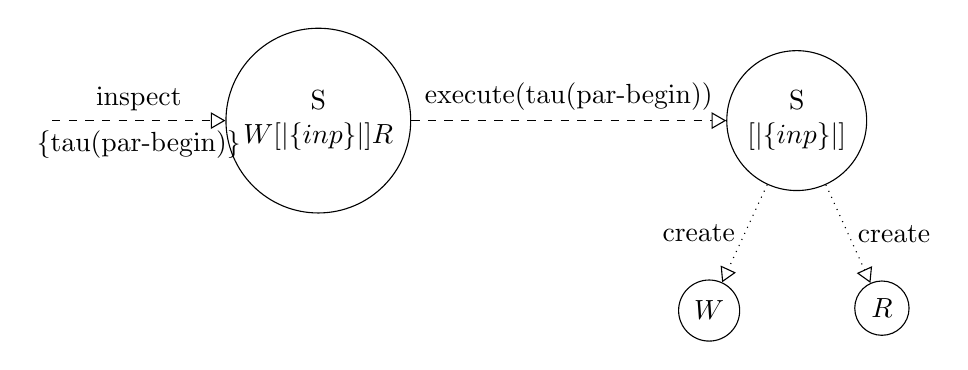
\begin{tikzpicture}[every text node part/.style={align=center}]
\tikzset{myFont/.style={font=\footnotesize}}
\tikzset{myBox/.style={draw,minimum height=1cm,myFont,text width=2.8cm}}
\tikzset{myGray/.style={fill=gray!10}}

\node[draw=none] (env) {};
\node[draw,circle,right=2.2cm of env] (parallel1) {S\\$W[|\{inp\}|]R$};
\path[draw,dashed,-open triangle 60] (env) edge node[above]{inspect} node[below]{\{tau(par-begin)\}} (parallel1);

\node[draw,circle, right=4cm of parallel1] (parallel2) {S\\$[|\{inp\}|]$};
\node[draw,circle,below left=1.5cm and .2 cm of parallel2] (W) {$W$};
\node[draw,circle,below right=1.5cm and .2 cm of parallel2] (R) {$R$};
\path[draw,dotted,-open triangle 60] (parallel2) edge node[left] {create} (W);
\path[draw,dotted, -open triangle 60] (parallel2) edge node[right] {create} (R);

\path[draw,dashed,-open triangle 60] (parallel1) edge node[above]{execute(tau(par-begin))} (parallel2);
\end{tikzpicture}
\captionof{figure}{Initial step of \autoref{lst:cmlexample} with process S as entry point.}
\label{fig:cmlmodel_first_step}
 \end{minipage} 

The inspection phase determines the possible transitions that are
available in the next step of execution. The result of the inspection
is shown as a set of transitions below ``inspect''. As seen on figure
\autoref{fig:cmlmodel_first_step} process P starts out by pointing to
the parallel composition constructs, this construct has a semantic
begin rule which does the initialization needed. In the figure
\autoref{fig:cmlmodel_first_step} that rule is named tau(par-begin)
and is therefore returned from the inspection. The reason for the name
tau(..) is that transitions can be either observable or silent, so in
principle any tau transition is not observable from the outside of the
process. However, in the interpreter all transitions flows out of the
inspection phase. When the inspection phase has completed, the
execution phase begins. The execution phase executes one of the
transitions returned from the inspection phase. In this case, only a
single transition is available so the tau(par-begin)) is executed
which creates the two child processes. The result of each of the shown
steps are the first configuration shown in the next step. So in this
case the resulting process configuration of
\autoref{fig:cmlmodel_first_step} is shown in figure
\autoref{fig:cmlmodel_second_step}.


The second step on \autoref{fig:cmlmodel_second_step} has a more
interesting inspection phase. According to the parallel composition
rule, we have that any event on the $inp$ channel must be
synchronized, meaning that W and R must only perform transition that
involves $inp$ channel events synchronously.


 \begin{minipage}{1\linewidth} 
  \centering %
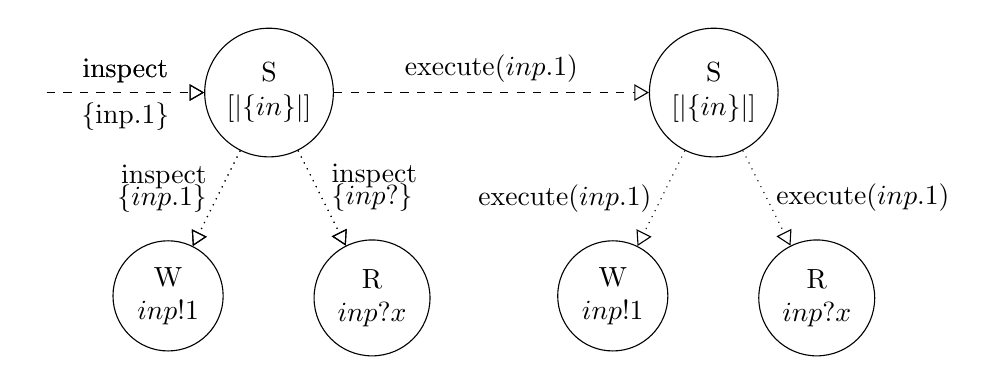
\begin{tikzpicture}[every text node part/.style={align=center}]
\tikzset{myFont/.style={font=\footnotesize}}
\tikzset{myBox/.style={draw,minimum height=1cm,myFont,text width=2.8cm}}
\tikzset{myGray/.style={fill=gray!10}}

\node[draw=none] (env) {};
\node[draw,circle,right=2cm of env] (parallel1) {S\\$[|\{in\}|]$};
\node[draw,circle,below left=1.5cm and .2 cm of parallel1] (W1) {W\\$inp!1$};
\node[draw,circle,below right=1.5cm and .2 cm of parallel1] (R1) {R\\$inp?x$};
\path[draw,dotted,-open triangle 60] (parallel1) edge node[above left] {inspect} (W1);
\path[draw,dotted,-open triangle 60] (parallel1) edge node[left] {$\{inp.1\}$} (W1);
\path[draw,dotted,-open triangle 60] (parallel1) edge node[above right] {inspect} (R1);
\path[draw,dotted,-open triangle 60] (parallel1) edge node[right] {$\{inp?\}$} (R1);

\path[draw,dashed,-open triangle 60] (env) edge node[above]{inspect} (parallel1);
\path[draw,dashed,-open triangle 60] (env) edge node[above]{inspect} node[below]{\{inp.1\}} (parallel1);

\node[draw,circle, right=4cm of parallel1] (parallel2) {S\\$[|\{in\}|]$};
\node[draw,circle,below left=1.5cm and .2 cm of parallel2] (W2) {W\\$inp!1$};
\node[draw,circle,below right=1.5cm and .2 cm of parallel2] (R2) {R\\$inp?x$};
\path[draw,dotted,-open triangle 60] (parallel2) edge node[left]{execute($inp.1$)} (W2);
\path[draw,dotted,-open triangle 60] (parallel2) edge node[right]{execute($inp.1$)} (R2);

\path[draw,dashed,-open triangle 60] (parallel1) edge node[above]{execute($inp.1$)} (parallel2);
\end{tikzpicture}
\captionof{figure}{Second step of \autoref{lst:cmlexample} with S as entry point.}
\label{fig:cmlmodel_second_step}
 \end{minipage} 

Therefore, when P is inspected it must inspect its child processes to
determine the possible transitions. In this case W can perform the
$inp.1$ event and R can perform any event on $inp$ and therefore, the
only possible transition is the one that performs the $inp.1$
event. This is then given to the execution phase which result in the
$inp.1$ event and moves both child processes into their next state.

\begin{minipage}{1\linewidth} 
  \centering %
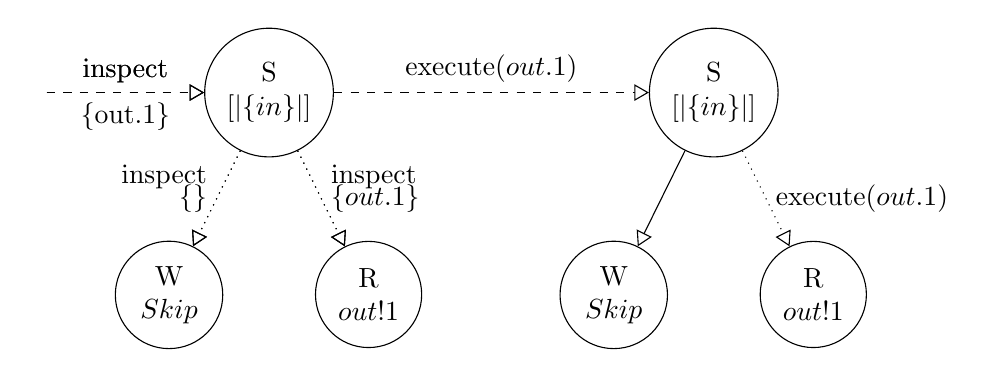
\begin{tikzpicture}[every text node part/.style={align=center}]
\tikzset{myFont/.style={font=\footnotesize}}
\tikzset{myBox/.style={draw,minimum height=1cm,myFont,text width=2.8cm}}
\tikzset{myGray/.style={fill=gray!10}}

\node[draw=none] (env) {};
\node[draw,circle,right=2cm of env] (parallel1) {S\\$[|\{in\}|]$};
\node[draw,circle,below left=1.5cm and .2 cm of parallel1] (W1) {W\\$Skip$};
\node[draw,circle,below right=1.5cm and .2 cm of parallel1] (R1) {R\\$out!1$};
\path[draw,dotted,-open triangle 60] (parallel1) edge node[above left] {inspect} (W1);
\path[draw,dotted,-open triangle 60] (parallel1) edge node[left] {$\{\}$} (W1);
\path[draw,dotted,-open triangle 60] (parallel1) edge node[above right] {inspect} (R1);
\path[draw,dotted,-open triangle 60] (parallel1) edge node[right] {$\{out.1\}$} (R1);

\path[draw,dashed,-open triangle 60] (env) edge node[above]{inspect} (parallel1);
\path[draw,dashed,-open triangle 60] (env) edge node[above]{inspect} node[below]{\{out.1\}} (parallel1);


\node[draw,circle, right=4cm of parallel1] (parallel2) {S\\$[|\{in\}|]$};
\node[draw,circle,below left=1.5cm and .2 cm of parallel2] (W2) {W\\$Skip$};
\node[draw,circle,below right=1.5cm and .2 cm of parallel2] (R2) {R\\$out!1$};
\path[draw,-open triangle 60] (parallel2) edge (W2);
\path[draw,dotted,-open triangle 60] (parallel2) edge node[right]{execute($out.1$)} (R2);

\path[draw,dashed,-open triangle 60] (parallel1) edge node[above]{execute($out.1$)} (parallel2);

\end{tikzpicture}
\captionof{figure}{Third step of \autoref{lst:cmlexample} with S as entry point}
\label{fig:cmlmodel_third_step}
 \end{minipage} 

In the third step on figure \autoref{fig:cmlmodel_third_step} W is now
Skip which means that it is successfully terminated. The inspection
for W therefore results in an empty set of possible transitions. R is
now waiting for the $out.1$ event after 1 was writting to $x$ in the
last step and therefore returns this transition. The execution phase
is a little different and S now knows only to execute R.

 \begin{minipage}{1\linewidth} 
  \centering %
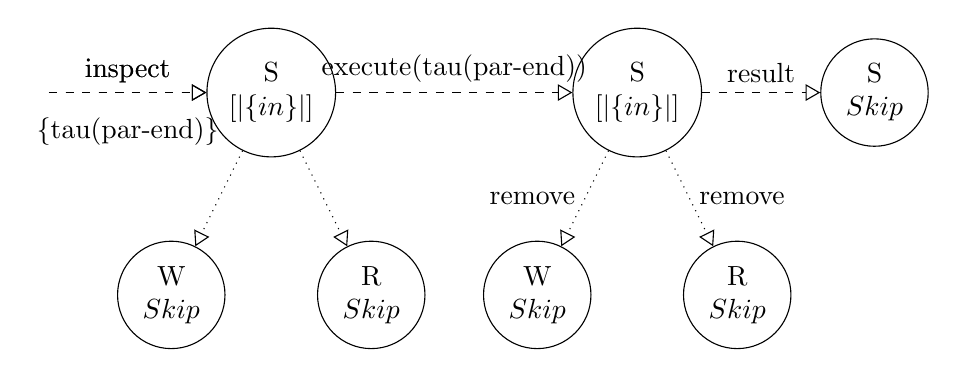
\begin{tikzpicture}[every text node part/.style={align=center}]
\tikzset{myFont/.style={font=\footnotesize}}
\tikzset{myBox/.style={draw,minimum height=1cm,myFont,text width=2.8cm}}
\tikzset{myGray/.style={fill=gray!10}}

\node[draw=none] (env) {};
\node[draw,circle,right=2cm of env] (parallel1) {S\\$[|\{in\}|]$};
\node[draw,circle,below left=1.5cm and .2 cm of parallel1] (W1) {W\\$Skip$};
\node[draw,circle,below right=1.5cm and .2 cm of parallel1] (R1) {R\\$Skip$};
\path[draw,dotted,-open triangle 60] (parallel1) edge (W1);
\path[draw,dotted,-open triangle 60] (parallel1) edge (R1);

\path[draw,dashed,-open triangle 60] (env) edge node[above]{inspect} (parallel1);
\path[draw,dashed,-open triangle 60] (env) edge node[above]{inspect} node[below=0.2cm]{\{tau(par-end)\}} (parallel1);


\node[draw,circle, right=3cm of parallel1] (parallel2) {S\\$[|\{in\}|]$};
\node[draw,circle,below left=1.5cm and .2 cm of parallel2] (W2) {W\\$Skip$};
\node[draw,circle,below right=1.5cm and .2 cm of parallel2] (R2) {R\\$Skip$};
\path[draw,dotted,-open triangle 60] (parallel2) edge node[left]{remove} (W2);
\path[draw,dotted,-open triangle 60] (parallel2) edge node[right]{remove} (R2);

\path[draw,dashed,-open triangle 60] (parallel1) edge node[above]{execute(tau(par-end))} (parallel2);

\node[draw,circle, right=1.5cm of parallel2] (parallel3) {S\\$Skip$};

\path[draw,dashed,-open triangle 60] (parallel2) edge node[above]{result} (parallel3);

\end{tikzpicture}
\captionof{figure}{Final step of \autoref{lst:cmlexample} where the parallel composition collapses unto a Skip process}
\label{fig:cmlmodel_fourth_step}
 \end{minipage} 

The fourth and final step shown in \autoref{fig:cmlmodel_fourth_step}
of the interpretation starts out with both W and R as Skip, this
triggeres the parallel end rules, which evolves into Skip. S therefore
returns the silent transition the triggers this end rule.

\subsection{Definitions}
\begin{description}
\item[CML] Compass Modelling Language
\item[UTP] Unified Theory of Programming, a semantic framework.
\item[Simulation] Simulation is when the interpreter runs without
  any form of user interaction other than starting and stoppping.
\item[Animation] Animation is when the user are involved in taking
  the decisions when interpreting the CML model
\end{description}

\section{Software Layers}
\label{sec:software_layers}
This section describes the layers of the CML
interpreter. As depicted in figure \ref{fig:layers} two highlevel layers exists.

\begin{figure}[ht!]
  \begin{center}
    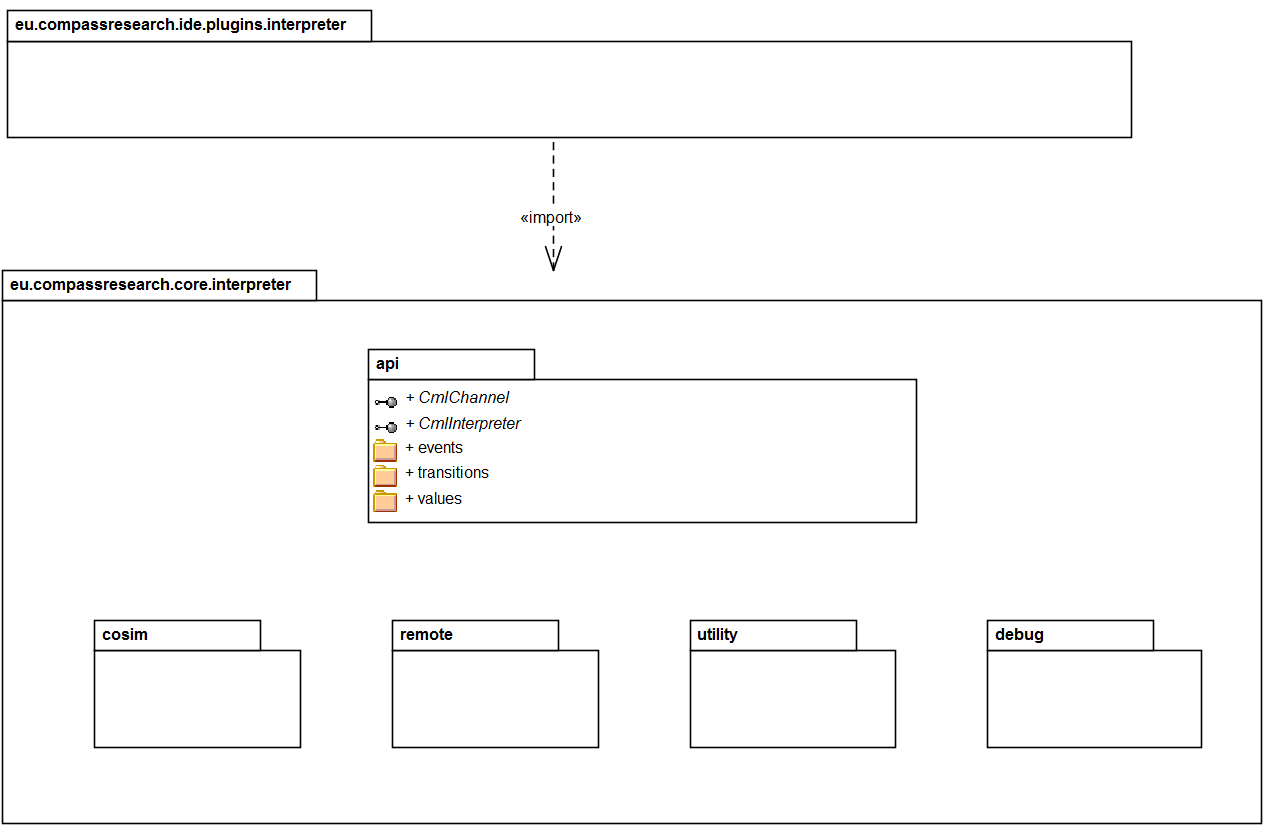
\includegraphics[width=1\textwidth]{figures/layers}
    \caption{The layers of the CML Interpreter}
    \label{fig:layers}
  \end{center}
\end{figure}

Each of these components will be described in further detail in the
following sections.

\subsection{The Core Layer}
This layer has the overall responsibility of interpreting a CML model
as described in the operational semantics that are defined in
\cite{D23.4} and is located in the java package named
\emph{eu.compassresearch.core.interpreter}. The design philosophy of
the top-level structure is to encapsulate all the classes and
interfaces that makes up the implementation of the core functionality
and only expose those that are needed to utilize the interpreter. This
provides a clean separation between the implementation and interface
and makes it clear for both the users, which not necessarily wants to
know about the implementation details, and developers which parts they
need to work with.

The following packages defines the top level structure of the core:
\begin{description}

\item[eu.compassresearch.core.interpreter] This package contains all
  the internal classes and interfaces that defines the core
  functionality of the interpreter. There is one important public class
  in the package, namely the \textbf{VanillaInterpreteFactory} factory
  class, that any user of the interpreter must invoke to use the
  interpreter. This can creates instances of the \textbf{CmlInterpreter}
  interface.
  
\item[eu.compassresearch.core.interpreter.api] This package and
  sub-packages contains all the public classes and interfaces that
  defines the API of the interpreter. This package includes the main
  interpreter interface \textbf{CmlInterpreter} along with the interface
  \textbf{CmlBehaviour} that represents any process or action, it
  corrosponds to the circles in \autoref{sec:problem_domain}




all the components that e any CML behavior. A CML
  behaviour is either an observable event like a channel synchronization
  or a internal event like a change of state. The main interface here is
  \textbf{CmlBehaviour} which can represent both a CML process and action.

  The api sub-packages groups the rest of the API classes and
  interfaces according to the responsibility they have.

\item[eu.compassresearch.core.interpreter.api.events] This package
  contains all the public components that enable users of the
  interpreter to subscribe to multiple on events (this it not CML
  channel events) from both \textbf{CmlIntepreter} and
  \textbf{CmlBehaviour} instances.

\item[eu.compassresearch.core.interpreter.api.transitions] This
  package contains all the possible types of transitions that a
  \textbf{CmlBehaviour} instance can make. This will be explained in
  more detail in section \ref{sec:transition_model}.

\item[eu.compassresearch.core.interpreter.api.values] This package
  contains all the values used in the CML interpreter. Values are used
  to represent the the result of an expression or the current state of a
  variable.

\item[eu.compassresearch.core.interpreter.debug] TBD

\item[eu.compassresearch.core.interpreter.utility] The utility
  packages contains components that generally reusable classes and
  interfaces. 

\item[eu.compassresearch.core.interpreter.utility.events] This package
  contains components helps to implement the Observer pattern. 

\item[eu.compassresearch.core.interpreter.utility.messaging] This
  package contains general components to pass message along a stream.

\end{description}

The \textbf{eu.compassresearch.core.interpreter} package are split into several
folders, each representing a different logical component. The
following folders are present

\begin{description}
\item[behavior] This folder contains all the internal classes and
  interfaces that implements the CmlBehaviors. The Cml behaviors will be
  described in more detail in in section \ref{sec:static_structure}, but
  they are bassically implemented by CML AST visitor classes.
\end{description}

\subsection{The IDE Layer}

Has the responsibility of visualizing the outputs of
  a running interpretation a CML model in the Eclipse Debugger. It is
  located in the \emph{eu.compassresearch.ide.plugins.interpreter}
  package.
The IDE part is integrating the interpreter into Eclipse, enabling CML
models to be debugged/simulated/animated through the Eclipse
interface. In \autoref{fig:interpreter_debuggerDeployment} a
deployment diagram of the debugging structure is shown.

\begin{figure}[ht!]
  \begin{center}
    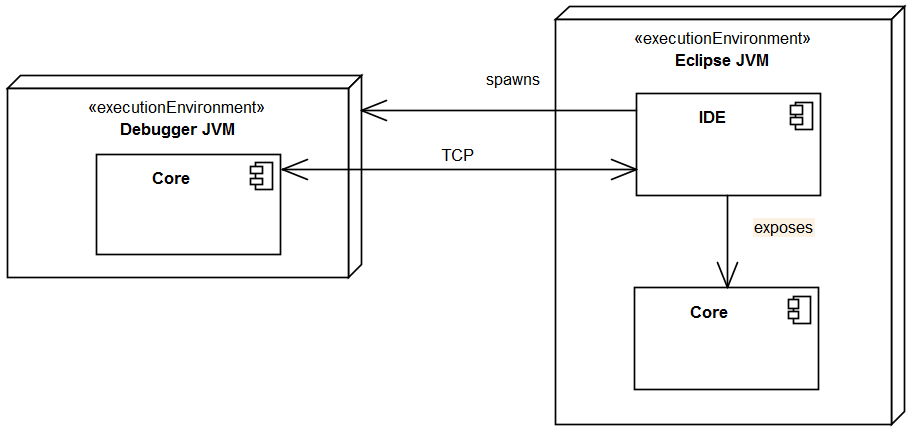
\includegraphics[width=1\textwidth]{figures/DebuggerDeploymentView}
    \caption{Deployment diagram of the debugger}
    \label{fig:interpreter_debuggerDeployment}
   \end{center}
\end{figure}

An Eclipse debugging session involves two JVMs, the one that the Eclipse
platform is executing in and one where only the Core executes in. All
communication between them is done via a TCP connection. 

Before explaining the steps involved in a debugging session, there are
two important classes worth mentioning:

\begin{itemize}
\item \textbf{CmlInterpreterController}: This is responsible for
  controlling the CmlInterpreter execution in the debugger JVM.  All
  communications to and from the interpreter handled in this class.
  
\item \textbf{CmlDebugTarget}: This class is part of the Eclipse
  debugging model. It has the responsiblity of representing a running
  interpreter on the Eclipse JVM side. All communications to and from
  the Eclipse debugger are handled in this class.
\end{itemize}

A debugging session has the following steps:
\begin{enumerate}
\item The user launches a debug session
\item On the Eclipse JVM a \textbf{CmlDebugTarget} instance is
  created, which listens for an incomming TCP connection.
\item A Debugger JVM is spawned and a
  \textbf{CmlInterpreterController} instance is created.
\item The \textbf{CmlInterpreterController} tries to connect to the
  created connection.
\item When the connection is established, the
  \textbf{CmlInterpreterController} instance will send a STARTING status
  message along with additional details
\item The \textbf{CmlDebugTarget} updates the GUI accordingly.
\item When the interpreter is running, status messages will be sent from \textbf{CmlInterpreterController} and commands and request messages are sent from \textbf{CmlDebugTarget}
\item This continues until \textbf{CmlInterpreterController} sends the STOPPED message
\end{enumerate}

TBD...
% \subsection{Subsection}
% \label{sec:subsection-1.1}

\section{Layer design and Implementation}
This section describes the static and dynamic structure of the
components involved in simulating/animating a CML model.

\subsection{Core Layer}

\subsubsection{Static Model}
\label{sec:static_structure}
The top level interface of the interpreter is depicted in figure
\ref{fig:interpreter_topLevelStructure}, followed by a short
description of each the depicted components.
\begin{figure}[ht!]
  \begin{center}
    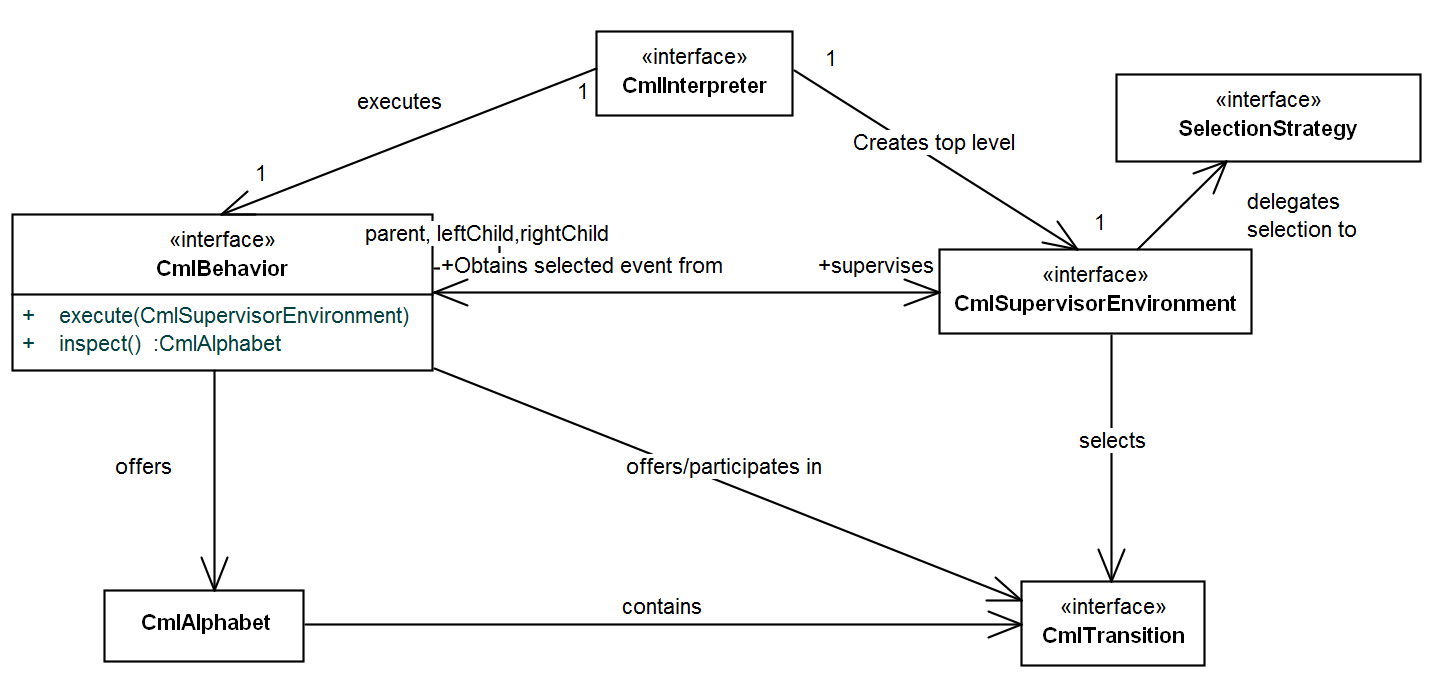
\includegraphics[width=1\textwidth]{figures/toplevelStructure}
    \caption{The high level classes and interfaces of the interpreter core component}
    \label{fig:interpreter_topLevelStructure}
  \end{center}
\end{figure}

\begin{description}
\item[CmlInterpreter] The main interface exposed by
  the interpreter component. This interface has the overall
  responsibility of interpreting. It exposes methods to execute, listen
  on interpreter events and get the current state of the interpreter. It
  is implemented by the \textbf{VanillaCmlInterpreter} class.
\item[CmlBehaviour] Interface that represents a behaviour specified by
  either a CML process or action. It exposes two methods: \emph{inspect}
  which calculates the immediate set of possible transitions that the
  current behaviour allows and \emph{execute} which takes one of the
  possible transitions determined by the supervisor. A specific
  behaviour can for instance be the prefix action ``a -> P'', where the
  only possible transition is to interact in the a event.  in any
\item [CmlSupervisorEnvironment] Interface with the responsibility of
  acting as the supervisor environment for CML processes and actions. A
  supervisor environment selects and exposes the next transition/event
  that should occur to its pupils (All the CmlBehaviors under its
  supervision). It also resolves possible backtracking issues which
  may occur in the internal choice operator. 
\item[SelectionStrategy] This interface has the responsibility
  of choosing an event from a given CmlAlphabet. This responsibility is
  delegated by the CmlSupervisorEnvironment interface.
\item[CmlTransition] Interface that represents any kind of transition that
  a CmlBehavior can make. This structure will be described in more
  detail in section \ref{sec:event_structure}.
\item[CmlAlphabet] This class is a set of CmlTransitions. It exposes
  convenient methods for manipulating the set.
\end{description}

To gain a better understanding of figure
\ref{fig:interpreter_topLevelStructure} a few things needs
mentioning. First of all any CML model (at least for now) has a top
level Process. Because of this, the interpreter need only to interact
with the top level CmlBehaviour instance. This explains the one-to-one
correspondence between the CmlInterpreter and the
CMLBehaviour. However, the behavior of top level CmlBehaviour is
determined by the binary tree of CmlBehaviour instances that itself
and it's child behaviours defines. So in effect, the CmlInterpreter
controls every transition that any CmlBehaviour makes through the top
level behaviour.

\subsubsection{Transition Model}
\label{sec:transition_model}

As described in the previous section a CML model is represented by a
binary tree of CmlBehaviour instances and each of these has a set of
possible transitions that they can make. A class diagram of all the
classes and interfaces that makes up transitions are shown in figure
\ref{fig:events}, followed by a description of each of the elements.

A transition taken by a CmlBehavior is represented by a
CMLTransition. This represent a possible next step in the model which can be either observable or silent (also called a tau
transition). 

An observable transition represents either that time passes or that a
communication/synchronization event takes place on a given
channel. All of these transitions are captured in the
ObservableTransition interface.  A silent transitions is captured by
the TauTransition and HiddenTransition class and can respectively
marks the occurrence of a an internal transition of a behavior or a
hidden channel transition.

\begin{figure}[ht!]
  \begin{center}
    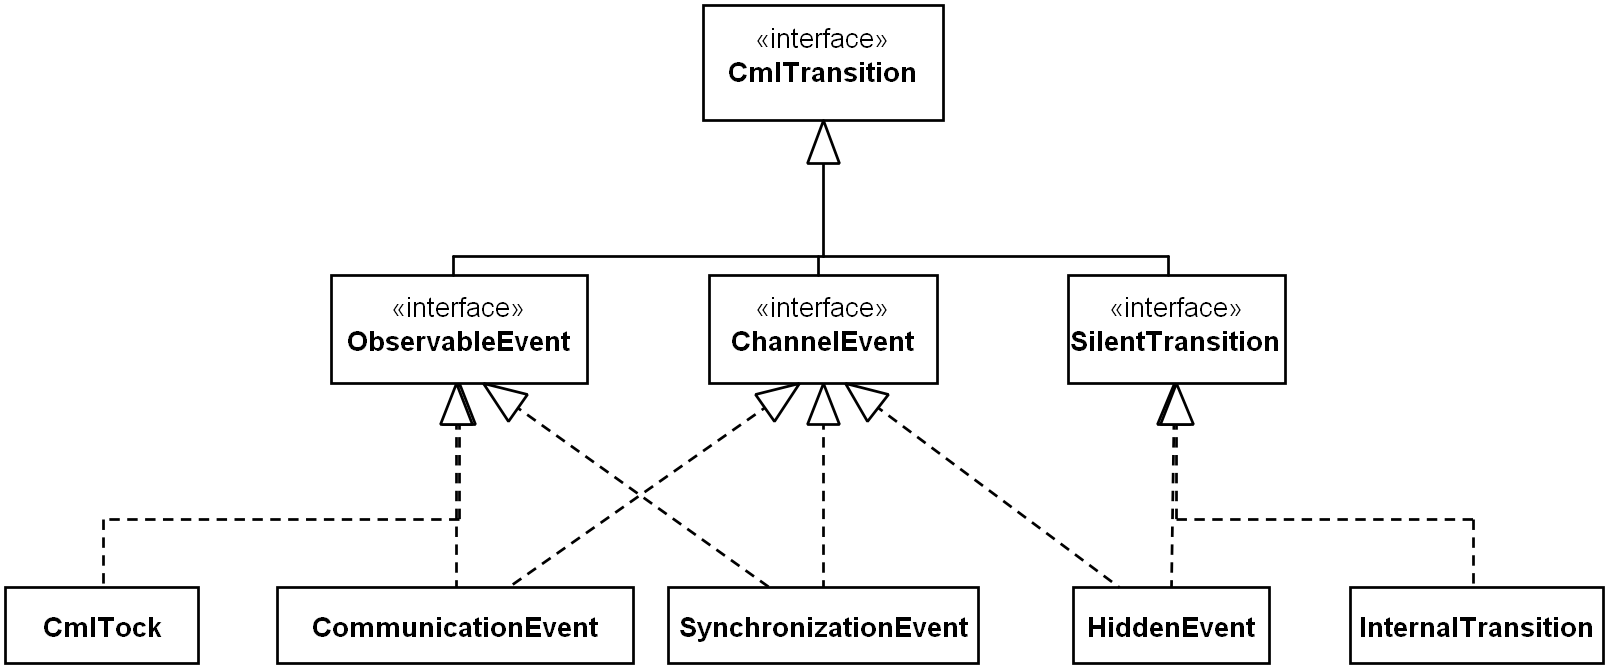
\includegraphics[width=1\textwidth]{figures/Events}
    \caption{The classes and interfaces that defines transitions/events}
    \label{fig:events}
  \end{center}
\end{figure}

\begin{description}
\item[CmlTransition] Represents any possible transition.
\item[CmlTransitionSet] Represents a set of CmlTransition objects.  
\item[ObservableTransition] This represents any observable transition.
\item[LabelledTransition] This represents any transition that results
  in a observable channel event
\item[TimedTransition] This represents a tock event marking the
  passage of a time unit.
\item[ObservableLabelledTransition] This represents the occurrence of
  a observable channel event which can be either a communication event
  or a synchronization event.
\item[TauTransition] This represents any non-observable transitions
  that can be taken in a behavior.
\item[HiddenEvent] This represents the occurrence of a hidden
  channel event in the form of a tau transition.
\end{description}

\subsubsection{Action/Process Structure}
\label{sec:action_process_structure}
Actions and processes are both represented by the CmlBehaviour
interface. A class diagram of the important classes that implements
this interface is shown in figure \ref{fig:cmlbehaviors}
\begin{figure}[ht!]
  \begin{center}
    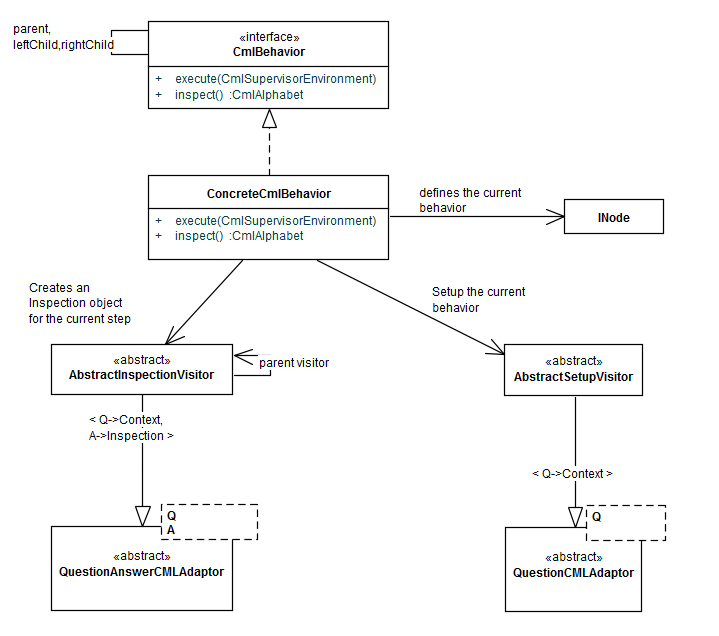
\includegraphics[width=0.9\textwidth]{figures/CmlBehaviors}
    \caption{The implementing classes of the CmlBehavior interface}
    \label{fig:cmlbehaviors}
  \end{center}
\end{figure}

As shown the \textbf{ConcreteCmlBehavior} is the implementing class of
the CmlBehavior interface. However, it delegates a large part of its
responsibility to other classes. The actual behavior of a
ConcreteCmlBehavior instance is decided by its current instance of the
INode interface, so when a ConcreteCmlBehavior instance is created a
INode instance must be given. The INode interface is implemented by
all the CML AST nodes and can therefore be any CML process or action.
The actual implementation of the behavior of any process/action is
delegated to three different kinds of visitors all extending a
generated abstract visitor that have the infrastructure to visit any
CML AST node.

The following three visitors are used:  
\begin{description}
\item[AbstractSetupVisitor] This has the responsibility of performing
  any required setup for every behavior. This visitor is invoked
  whenever a new INode instance is loaded.

\item[AbstractEvaluationVisitor] This has the responsibility of
  performing the actual behavior and is invoked inside the \textbf{execute}
  method. This involves taking one of the possible transitions.

\item[AbstractAlphabetVisitor] This has the responsibility of
  calculating the alphabet of the current behavior and is invoked in the
  \textbf{inspect} method.
\end{description}

In figure \ref{fig:visitors} a more detailed look at the evaluation visitor structure is given.  

\begin{figure}[ht!]
  \begin{center}
    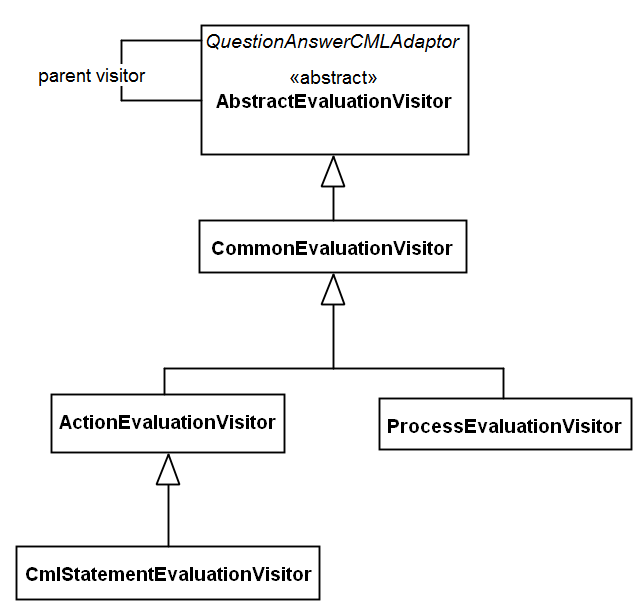
\includegraphics[width=1\textwidth]{figures/Visitors}
    \caption{Visitor structure}
    \label{fig:visitors}
  \end{center}
\end{figure}

As depicted the visitors are split into several visitors that handle
different parts of the languages. The sole reason for doing this is to
avoid having one large visitor that handles all the cases. At run-time
the visitors are setup in a tree structure where the top most visitor
is a \textbf{CmlEvaluationVisitor} instance which then delegates to
either a \textbf{ActionEvaluationVisitor} and
\textbf{ProcessEvaluationVisitor} etc.


\subsubsection{Dynamic Model}
\label{sec:dynamic_structure}

The previous section described the high-level static structure, this
section will describe the high-level dynamic structure.

First of all, the entire CML interpreter runs in a single thread. This
is mainly due to the inherent complexity of concurrent
programming. You could argue that since a large part of COMPASS is
about modelling complex concurrent systems, we also need a concurrent
interpretation of the models. However, the semantics is perfectly
implementable in a single thread which makes a multi-threaded
interpreter optional. There are of course benefits to a multi-threaded
interpreter such as performance, but for matters such as the testing
and deterministic behaviour a single threaded interpreter is much
easier to handle and comprehend.

To start a simulation/animation of a CML model, you first of all need
an instance of the \textbf{CmlInterpreter} interface. This is created
through the \textbf{VanillaInterpreterFactory} by invoking the
\textbf{newInterpreter} method with a typechecked AST of the CML
model. The currently returned implementation is the
\textbf{VanillaCmlInterpreter} class. Once a \textbf{CmlInterpreter}
is instantiated the interpretation of the CML model is started
by invoking the \textbf{execute} method given a
\textbf{CmlSupervisorEnvironment}.

In figure \ref{fig:dynamic_toplevel} a high level sequence diagram of
the \textbf{execute} method on the \textbf{VanillaCmlInterpreter}
class is depicted. 

\begin{figure}[ht!]
  \begin{center}
    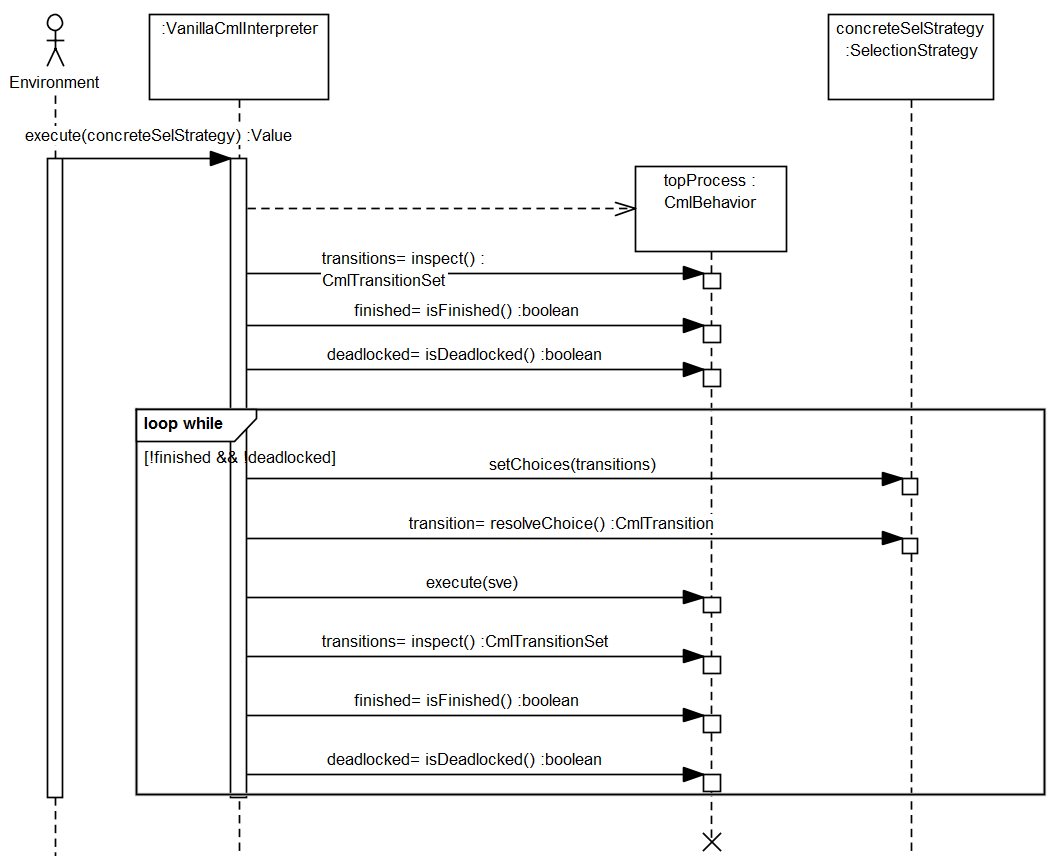
\includegraphics[width=1\textwidth]{figures/DynamicTopLevel}
    \caption{The top level dynamics}
    \label{fig:dynamic_toplevel}
  \end{center}
\end{figure}

As seen in the figure the model is executed until the top level
process is either successfully terminated or deadlocked. For each 

\subsubsection{CmlBehaviors}

As explained in section \ref{} the CmlBehavior instances forms a binary tree at runtime. 


\subsection{The IDE Layer}
\label{sec:user_interface}

%%%% Bibliography %%%%
\newpage
\bibliographystyle{alpha}
\bibliography{bibliography} 
\label{ch:bib} %label to refer to


\end{document}  